\documentclass[]{../sty/JGCD}
\usepackage{%
  float,
  amssymb,
  amsmath,
  indentfirst,
  booktabs,
  empheq,
  enumerate,
  amsthm,
  thmtools,
  array,
  longtable,
  setspace,
  amsmath,
  times
}
\usepackage[compact]{titlesec}
\usepackage[titles]{tocloft}
\usepackage[shortlabels]{enumitem}
\usepackage[english]{babel}

\newcommand{\figurepath}{../fig}
\newcommand{\bibsourcepath}{../bib/aiaa-jgcd-2015}

% Theorem styles
\declaretheoremstyle[
  headfont=\bfseries,
  notebraces={}{},
  notefont=\bfseries,
  bodyfont=\itshape,
  headpunct={},
  headformat={\hspace{0.0in}\makebox[0.65in][l]{\NAME\ \NUMBER\ }{\NOTE}}\hspace{0.1in}
]{thm-style-1}

\declaretheoremstyle[
  headfont=\bfseries,
  notebraces={}{},
  notefont=\bfseries,
  bodyfont=\itshape,
  headpunct={},
  headformat={\hspace{0.0in}\makebox[0.65in][l]{\NAME\ \NUMBER\ }{\NOTE}}\hspace{0.1in}
]{lem-style-1}

\declaretheoremstyle[
  headfont=\bfseries,
  notebraces={}{},
  notefont=\bfseries,
  bodyfont=\itshape,
  headpunct={},
  headformat={\NAME\ \NUMBER\ }
]{cor-style-1}

\declaretheoremstyle[
  headfont=\scshape,
  notefont=\itshape,
  bodyfont=\normalfont,
  headpunct=\relax,
  headformat={\makebox[0.5in][r]{\NAME\ }\NOTE},
]{prf-style-1}

\declaretheoremstyle[
  headfont=\bfseries,
  notebraces={}{},
  notefont=\bfseries,
  headpunct={},headformat={\NAME\ \NOTE}
]{ass-style-1}

\declaretheoremstyle[
  headfont=\bfseries,
  notebraces={}{},
  notefont=\bfseries,
  headpunct={},
  headformat={\NAME\ \NUMBER\ }{\NOTE}
]{rem-style-1}

%Need to undeclare the proof environment that amsthm provides but I can't use \renewenvironment
\let\proof\relax
\let\endproof\relax

% Use these styles in definitions of proof, theorem, etc.
\declaretheorem[style=thm-style-1,numbered=yes,name=Theorem]{thm-dan}
\declaretheorem[style=lem-style-1,numbered=yes,name=Lemma]{lem-dan}
\declaretheorem[style=cor-style-1,numbered=no,name=Corollary]{cor-dan}
\declaretheorem[style=prf-style-1,name=Proof,qed=\qedsymbol]{proof-dan}
\declaretheorem[style=ass-style-1,numbered=yes,name=Assumption]{ass-dan}
\declaretheorem[style=rem-style-1,numbered=yes,name=Remark]{rem-dan}
\declaretheorem[style=rem-style-1,numbered=yes,name=Definition]{defn-dan}
\declaretheorem[style=rem-style-1,numbered=yes,name=Proposition]{prop-dan}

%------------------------------------------------------------------------------------------------------------------
%To allow bold symbols in section headings
\makeatletter
\g@addto@macro\bfseries{\boldmath}
\makeatother
%------------------------------------------------------------------------------------------------------------------

\newtheoremstyle{examplestyle}% name of the style to be used
{}% measure of space to leave above the theorem. E.g.: 3pt
{}% measure of space to leave below the theorem. E.g.: 3pt
{\slshape}% name of font to use in the body of the theorem
{0pt}% measure of space to indent
{\bfseries}% name of head font
{\vspace{-6pt}}% punctuation between head and body eg \newline
{0pt}% space after theorem head
{}% Manually specify head
\theoremstyle{examplestyle}
\newtheorem{innercustomthm}{Assumption}
\newenvironment{customthm}[1]
  {\renewcommand\theinnercustomthm{#1}\innercustomthm\normalfont}
  {\endinnercustomthm}

\begin{document}

  \title{Adaptive Output Feedback Based on Closed-Loop Reference Models for Hypersonic Vehicles}

  \author{Daniel P. Wiese\footnote{Graduate Student, Mechanical Engineering, 77 Massachusetts Ave. Rm 3--441, Student Member AIAA} and Anuradha M. Annaswamy\footnote{Senior Research Scientist, Mechanical Engineering, 77 Massachusetts Ave. Rm 3--348, Member AIAA}}
  \affiliation{Massachusetts Institute of Technology, Cambridge, MA 02139}
  \author{Jonathan A. Muse\footnote{Research Aerospace Engineer, Autonomous Control Branch, 2210 Eighth St., Senior Member AIAA} and Michael A. Bolender\footnote{Senior Aerospace Engineer, Autonomous Control Branch, 2210 Eighth St., Associate Fellow AIAA}}
  \affiliation{U.S. Air Force Research Laboratory, Wright-Patterson Air Force Base, Ohio 45433}
  \author{Eugene Lavretsky\footnote{Boeing Senior Technical Fellow, Associate Fellow AIAA}}
  \affiliation{The Boeing Company, Huntington Beach, CA 92647, USA}

  \begin{abstract}
    This paper presents a new method of synthesizing an output feedback adaptive controller for a class of uncertain, non-square, multi-input multi-output systems that often occur in hypersonic vehicle models.
    The main challenge that needs to be addressed is the determination of a corresponding square and strictly positive real transfer function.
    This paper proposes a new procedure to synthesize two gain matrices that allows the realization of such a transfer function, thereby allowing a globally stable adaptive output feedback law to be generated.

    The unique features of this output feedback adaptive controller are a baseline controller that uses a Luenberger observer, a closed-loop reference model, manipulations of a bilinear matrix inequality, and the Kalman-Yakubovich Lemma.
    Using these features, a simple design procedure is proposed for the adaptive controller, and the corresponding stability property is established.
    The proposed adaptive controller is compared to the classical multi-input multi-output adaptive controller.

    A numerical example based on a scramjet powered, blended wing-body generic hypersonic vehicle model is presented.
    The 6 degree-of-freedom nonlinear vehicle model is linearized, giving the design model for which the controller is synthesized.
    The adaptive output feedback controller is then applied to an evaluation model, which is nonlinear, coupled, and includes actuator dynamics, and is shown to result in stable tracking in the presence of uncertainties that destabilize the baseline linear output feedback controller.
  \end{abstract}

  \maketitle

  \section*{Nomenclature}
  \noindent
  \begin{longtable}[l]{@{}lcl@{}}
    $A$ &=& Nominal augmented open-loop state matrix \\
    $A_{m}$ &=& Reference model state matrix \\
    $A_{p}$ &=& Open-loop state matrix about nominal trim\\
    $\bar{A}$ &=& Transformed state matrix \\
    $\bar{A}_{ij}$ &=& Partition of transformed state matrix \\
    $B$ &=& Nominal augmented open-loop control input matrix \\
    $B_{\text{cmd}}$ &=& Nominal augmented open-loop reference input matrix \\
    $B_{p}$ &=& Open-loop input matrix about nominal trim \\
    $C$ &=& Nominal augmented open-loop measured output matrix \\
    $\bar{C}$ &=& Transformed output matrix partition \\
    $C_{p}$ &=& Open-loop measured output matrix about nominal trim \\
    $C_{pz}$ &=& Open-loop regulated output matrix about nominal trim \\
    $C_{s}$ &=& Post-compensated augmented state space output matrix \\
    $D_{pz}$ &=& Open-loop control feed-through matrix about nominal trim \\
    $E$ &=& Constant matrix \\
    $e_{s}$ &=& Synthetic output error \\
    $e_{x}$ &=& State tracking error \\
    $e_{y}$ &=& Measured output error \\
    $F$ &=& Matrix \\
    $G$ &=& Matrix \\
    $G(s)$ &=& Transfer matrix \\
    $H$ &=& Matrix \\
    $H_{i}$ &=& Markov parameters, where $i$ is equal to 0, 1, 2, \dots \\
    $H_{p}$ &=& Hermite form of transfer matrix \\
    $I$ &=& Identity matrix \\
    $J$ &=& Matrix \\
    $K$ &=& Matrix \\
    $K_{p}$ &=& High frequency gain matrix \\
    $K_{x}$ &=& Feedback gain \\
    $L$ &=& Closed-loop reference model gain \\
    $\ell$ &=& Dimension of measured output of open-loop plant \\
    $M$ &=& Output annihilator matrix \\
    $M_{0}$ &=& Transformed output annihilator matrix \\
    $m$ &=& Number of open-loop plant inputs \\
    $N$ &=& Input annihilator matrix \\
    $N_{1}$ &=& Matrix \\
    $N_{2}$ &=& Matrix \\
    $N_{0}$ &=& Transformed input annihilator matrix \\
    $n$ &=& Dimension of augmented plant state \\
    $n_{e}$ &=& Number of regulated outputs \\
    $n_{p}$ &=& Dimension of open-loop plant state \\
    $P$ &=& Positive definite matrix \\
    $p$ &=& Dimension of augmented open-loop plant measured output \\
    $p$ &=& Roll rate, deg/s \\
    $Q$ &=& Positive definite matrix \\
    $\widehat{Q}$ &=& Positive definite matrix \\
    $q$ &=& Pitch rate, deg/s \\
    $R$ &=& Matrix \\
    $r$ &=& Yaw rate, deg/s \\
    $\mathbb{R}_{p}(s)$ &=& Ring of proper rational transfer functions with coefficients in $\mathbb{R}$ \\
    $S_{1}$ &=& Augmented plant measured output postcompensator \\
    $T$ &=& Matrix \\
    $t$ &=& Time, s \\
    $U$ &=& Matrix \\
    $u$ &=& Control input \\
    $u_{\text{bl}}$ &=& Baseline control input \\
    $V(\cdot,\cdot)$ &=& Lyapunov candidate \\
    $W_{p}(s)$ &=& Transfer matrix \\
    $X$, $X_{11}$, $X_{22}$ &=& Positive definite matrix \\
    $x_{e}$ &=& Integral error state \\
    $x_{m}$ &=& Reference model state \\
    $x_{p}$ &=& System state linearized about nominal trim \\
    $y$ &=& Augmented open-loop plant measured output \\
    $y_{m}$ &=& Reference model measured output \\
    $y_{p}$ &=& Open-loop plant measured output \\
    $z$ &=& Open-loop plant regulated output \\
    $z_{\text{cmd}}$ &=& Regulated command input \\
    $\alpha$ &=& Angle of attack, deg \\
    $\beta$ &=& Sideslip angle, deg \\
    $\Gamma$ &=& Adaptive gain matrix \\
    $\delta_{a}$ &=& Aileron deflection angle, deg \\
    $\delta_{e}$ &=& Elevator deflection angle, deg \\
    $\delta_{r}$ &=& Rudder deflection angle, deg \\
    $\Theta$ &=& Adaptive parameter matrix \\
    $\widetilde{\Theta}$ &=& Adaptive parameter error \\
    $\Theta^{*}$ &=& Ideal adaptive parameter matrix \\
    $\Lambda$ &=& Control ineffectiveness uncertainty \\
    $\nu$ &=& Observability index \\
    $\Xi$ &=& Similarity transform matrix \\
    $\Sigma$ &=& State-space linear system \\
    $\phi$ &=& Roll angle, deg \\
    $\Psi$ &=& Augmented open-loop plant state matrix uncertainty \\
    $\Psi_{p}$ &=& Open-loop plant state matrix uncertainty \\
    $\Omega$ &=& Upper bound on state matrix uncertainty \\
  \end{longtable}

  \section{Introduction}\label{sec.intro}

  A state feedback linear quadratic regulator (LQR) baseline controller with integral action and augmented with an adaptive component has proven to be an effective choice for accommodating the parametric uncertainties present in flight control applications, and ensuring satisfactory reference tracking\ \cite{jang.adaptive.2007,gibson.adaptive.2008,matsutani.adaptivegtm.2009,crespo.adaptivegtm.2009,dydek.adaptivex15.2010,wiese.adaptive.2013,lavretskywise.book.2013}.
  However, such a controller requires that the state is measurable, which may not always be possible.
  Also, inaccuracies in the system output measurements may render state feedback controllers sensitive to measurement errors and thus not applicable.
  For these reasons there has been an increasing drive to develop an adaptive output feedback extension of the robust integral-augmented LQR baseline plus adaptive controller.

  Existing classical methods of multi-input multi-output (MIMO) output feedback adaptive control are applicable for plants that are square\ \cite{tao.multivariable.2014}.
  An $m\times m$ transfer matrix is used to represent the dynamic behavior of the plant, and the existence of a stable adaptive solution depends on the available prior information about this plant transfer matrix\ \cite{singh.prior.1984,narendra.stable.2005}.
  The solution relies on non-minimal controller representations to dynamically decouple the plant, and the controller structure consists of a feedforward gain and two filters in the feedback path, the order of which depends on $m$ and an upper bound on the observability index of the plant, $\nu$.
  The resulting classical MIMO adaptive solution will introduce $2m\nu$ controller states and $2m^{2}\nu$ adjustable parameters.

  More recent methods of MIMO output feedback adaptive control have adopted a Luenberger observer-based approach in which a \textit{minimal} observer is used to generate a state estimate to use for feedback control\ \cite{lavretsky.output.2010,wise.obltrdesign.2013,qu.gnc.2013,lavretskywise.book.2013}.
  This observer also serves as the reference model which is used by the adaptive controller, and the presence of the observer feedback gain $L$ provides the structure known as the closed-loop reference model, or CRM\ \cite{gibson.aiaacrm.2012,gibson.ecc.2013,gibson.ieeeaccess.2013,gibson.acc.2013}.
  These CRM based approaches have relied on the so-called squaring-up procedure\ \cite{misra.squareup.1992} to add fictitious inputs to a tall system (one where the dimension of the output is greater than the dimension of the input) making it square and ensuring any transmission zeros are stable.
  These fictitious inputs are used only to synthesize a postcompensator $S_{1}$ and the CRM gain $L$ which ultimately render a set of underlying error dynamics strictly positive real (SPR).
  These SPR error dynamics allowed stable update laws to be chosen to guarantee system stability.
  We note that systems with transmission zeros cannot be squared up using the method as described in Reference\ \cite{misra.squareup.1992}, which has led to a recent modification to overcome this limitation and allow the design of output feedback controllers for systems with stable transmission zeros\ \cite{quwiese.ifac.2014}.

  The CRM based output feedback design procedure proposed in this paper takes an alternative approach to synthesizing $S_{1}$ and $L$ which does not require the system first be squared-up.
  Instead, the postcompensator $S_{1}$ is determined as a generalized inverse of the system matrices, and a state feedback approach is used to stabilize a related lower order plant subsystem.
  This results in a feasible linear matrix inequality (LMI) which is solved to yield $L$.
  We consider in this work the case of tall systems, but the case of wide systems holds by duality.
  Furthermore, because $L$ is a component of both the baseline and adaptive controllers, it is crucial that it be selected to provide good frequency domain properties for the baseline control system, as well as desirable adaptive control performance.
  This procedure is able to exploit the structure of the given system to obtain a large amount of freedom in the selection of $L$ in order to achieve a robust baseline control design and the desired adaptive performance.

  In Section~\ref{sec.controlproblem} we introduce the class of uncertain plants which we wish to control, propose a control architecture, and formulate the control problem of interest.
  In Section~\ref{sec.preliminaries} we provide some preliminaries which will be used in the synthesis of a globally stable controller for the uncertain system.
  Section~\ref{sec.adaptivecontroldesign} provides a constructive procedure for obtaining an update law for an adaptive controller which guarantees global stability, and compares the proposed controller to the existing classical controller.
  Finally, a numerical example is presented in Section~\ref{sec.example} to illustrate the efficacy of this method when applied to a 6-DOF nonlinear generic hypersonic vehicle (GHV) model\ \cite{wiese.adaptive.2013,rollins.nonlinear.2013}.

  \section{Control Problem Formulation}\label{sec.controlproblem}

  Consider the following MIMO uncertain open-loop system
  \begin{equation}
    \label{eqn.openloopsystem}
    \begin{split}
      \dot{x}_{p}&=A_{p}x_{p}+B_{p}(\Lambda u+\Psi_{p}^{\top}x_{p}) \\
      y_{p}&=C_{p}x_{p} \\
      z&=C_{pz}x_{p}+D_{pz}(\Lambda u+\Psi_{p}^{\top}x_{p})
    \end{split}
  \end{equation}
  where $A_{p}\in\mathbb{R}^{n_{p}\times n_{p}}$, $B_{p}\in\mathbb{R}^{n_{p}\times m}$, $C_{p}\in\mathbb{R}^{\ell\times n_{p}}$, $C_{pz}\in\mathbb{R}^{n_{e}\times n_{p}}$, $D_{pz}\in\mathbb{R}^{n_{e}\times m}$ are constant \textit{known} matrices.
  The nonsingular matrix $\Lambda\in\mathbb{R}^{m\times m}$ and $\Psi_{p}\in\mathbb{R}^{m\times n_{p}}$, which represents constant matched uncertainty weights that enter the system through the columns of $B_{p}$, are \textit{unknown}.
  The \textit{measured} output is $y_{p}$, the \textit{regulated} output is $z$, and the number of regulated outputs cannot exceed the number of inputs, that is $n_{e}\leq m$.
  The goal is to design a control input $u$ which will make $z$ track the reference command $z_{\text{cmd}}$ with bounded errors in the presence of the uncertainties $\Lambda$ and $\Psi_{p}$.
  A typical example of\ \eqref{eqn.openloopsystem} in flight control corresponds to the tracking of a body acceleration command in the presence of uncertainties in stability and control derivatives.
  We make the following assumptions about the system in Eq.\ \eqref{eqn.openloopsystem}.

  \begin{customthm}{1} $\;$\label{ass.plant}
    \begin{enumerate}[\Alph{enumi}), ref=\Alph{enumi}] %chktex 9 chktex 10
    \itemsep0em
    \item{$(A_{p},B_{p})$ is controllable.\label{ass.p.cont}}
    \item{$(A_{p},C_{p})$ is observable.\label{ass.p.obsv}}
    \item{$B_{p}$, $C_{p}$, and $C_{p}B_{p}$ are full rank.\label{ass.p.rank}}
    \item{Any finite transmission zeros of $(A_{p},B_{p},C_{p},0)$ are strictly stable, and the rank of the following matrix is full\label{ass.p.tzero}}
    \begin{equation*}
      \text{rank}\left(
      \begin{bmatrix}
        A_{p} & B_{p} \\
        -C_{pz} & D_{pz}
      \end{bmatrix}\right)
      =n_{p}+n_{e}
    \end{equation*}
    \item{%
      \begin{enumerate}[(\alph{enumii}), ref=\alph{enumii}]
        \item{$\Lambda$ is nonsingular and diagonal with entries of known sign\label{ass.p.unc.lambda}}
        \item{$\|\Psi_{p}\|_{2}<\Omega<\infty$, where $\Omega$ is known\label{ass.p.unc.wp}}
      \end{enumerate}\label{ass.p.unc}
    }
    \end{enumerate}
  \end{customthm}

  In order to facilitate command tracking, we introduce integral action, and for this purpose an additional state $x_e$ is defined as
  \begin{equation}
    \label{eqn.xedot}
    \dot{x}_{e}=z_{\text{cmd}}-z
  \end{equation}
  This integral error state is appended to the plant in Eq.\ \eqref{eqn.openloopsystem} leading to the following augmented open-loop dynamics
  \begin{equation}
    \label{eqn.uncsystemfull}
    \begin{split}
      \begin{bmatrix}
        \dot{x}_{p} \\
        \dot{x}_{e}
      \end{bmatrix}
      &=
      \begin{bmatrix}
        A_{p} & 0 \\
        -C_{pz} & 0
      \end{bmatrix}
      \begin{bmatrix}
        x_{p} \\
        x_{e}
      \end{bmatrix}
      +
      \begin{bmatrix}
        B_{p} \\
        -D_{pz}
      \end{bmatrix}(\Lambda u+\Psi_{p}^{\top}x_{p})
      +
      \begin{bmatrix}
        0 \\
        I
      \end{bmatrix}z_{\text{cmd}} \\
      \begin{bmatrix}
        y_{p} \\
        x_{e}
      \end{bmatrix}
      &=
      \begin{bmatrix}
        C_{p} & 0 \\
        0 & I
      \end{bmatrix}
      \begin{bmatrix}
        x_{p} \\
        x_{e}
      \end{bmatrix} \\
    \end{split}
  \end{equation}
  The system in Eq.\ \eqref{eqn.uncsystemfull} can be written more compactly as follows
  \begin{equation}
    \label{eqn.uncsystem}
    \begin{split}
      \dot{x}&=Ax+B(\Lambda u+\Psi^{\top}x)+B_{\text{cmd}}z_{\text{cmd}} \\
      y&=Cx
    \end{split}
  \end{equation}
  where $\Sigma=(A,B,C,0)$, and where $A\in\mathbb{R}^{n\times n}$, $B\in\mathbb{R}^{n\times m}$, $B_{\text{cmd}}\in\mathbb{R}^{n\times n_{e}}$, and $C\in\mathbb{R}^{p\times n}$ are the known matrices given by
  \begin{equation*}
    A=
    \begin{bmatrix}
      A_{p} & 0_{n_{p}\times n_{e}} \\
      -C_{pz} & 0_{n_{e}\times n_{e}}
    \end{bmatrix} \quad
    B=
    \begin{bmatrix}
      B_{p} \\
      -D_{pz}
    \end{bmatrix}
    \quad
    B_{\text{cmd}}=
    \begin{bmatrix}
      0_{n_{p}\times m} \\
      I_{n_{e}\times n_{e}}
    \end{bmatrix}
    \quad
    C=
    \begin{bmatrix}
      C_{p} & 0_{\ell\times n_{e}} \\
      0_{n_{e}\times n_{p}} & I_{n_{e}\times n_{e}}
    \end{bmatrix}
  \end{equation*}
  and where $\Psi=[\;\Psi_{p}^{\top}\;\;0_{m\times n_{e}}\;]^{\top}$ is unknown. Note that $p=\ell+n_{e}$. It can be shown that Assumption~\ref{ass.plant} regarding the plant in Eq.\ \eqref{eqn.openloopsystem} is equivalent to Assumption~\ref{ass.uncsystem} regarding the system $\Sigma$ in\ \eqref{eqn.uncsystem}, which is stated below.

  \begin{customthm}{$1^{\prime}$} $\;$\label{ass.uncsystem}
    \begin{enumerate}[\Alph{enumi}), ref=\Alph{enumi}] %chktex 9 chktex 10
      \itemsep0em
      \item{$(A,B)$ is controllable.\label{ass.cont}}
      \item{$(A,C)$ is observable.\label{ass.obsv}}
      \item{$B$, $C$, and $CB$ are full rank.\label{ass.rank}}
      \item{Any finite transmission zeros of $(A,B,C,0)$ are strictly stable.\label{ass.tzero}}
      \item{%
        \begin{enumerate}[(\alph{enumii}), ref=\alph{enumii}]
          \item{$\Lambda$ is nonsingular and diagonal with entries of known sign\label{ass.unc.lambda}}
          \item{$\|\Psi\|_{2}<\Omega<\infty$, where $\Omega$ is known\label{ass.unc.w}}
        \end{enumerate}\label{ass.unc}
      }
      \item{$\Sigma$ is tall: $p>m$.\label{ass.tall}}
    \end{enumerate}
  \end{customthm}

  \begin{rem-dan}
    The system in Eq.\ \eqref{eqn.openloopsystem} satisfying Assumption~\ref{ass.plant}\ref{ass.p.cont}-\ref{ass.p.tzero} when augmented with the integral error state as shown in Eq.\ \eqref{eqn.uncsystemfull} also satisfies Assumption~\ref{ass.uncsystem}\ref{ass.cont}-\ref{ass.tzero}.
    In other words, under Assumption~\ref{ass.plant}\ref{ass.p.cont}-\ref{ass.p.tzero}, integral error augmentation does not destroy controllability, observability, or the rank conditions.
    Nor does it add any transmission zeros\ \cite{lavretsky.output.2010}.
  \end{rem-dan}

  \begin{rem-dan}
    Assumptions~\ref{ass.uncsystem}\ref{ass.cont} and~\ref{ass.uncsystem}\ref{ass.obsv} are standard. Assumption~\ref{ass.uncsystem}\ref{ass.rank} implies that inputs and outputs are not redundant, as well as a MIMO equivalent of relative degree unity.
    Assumption~\ref{ass.uncsystem}\ref{ass.tzero} is a standard requirement for output feedback adaptive control.
    Assumption~\ref{ass.uncsystem}\ref{ass.tall} can be considered without loss of generality as the case of wide systems $p<m$ holds by duality.
    The case of square systems has been given in Reference\ \cite{huang.designspr.1999} and is discussed in Section~\ref{sec.adaptivecontroldesign}.
  \end{rem-dan}

  \subsection{Baseline Control Design}

  The underlying problem here is to design a control input $u$ in Eq.\ \eqref{eqn.uncsystem} so that the closed-loop system has bounded solutions and $z$ tends to  $z_{{\rm cmd}}$ with bounded errors in the presence of the uncertainties $\Lambda$ and $\Psi$.
  In this section, we describe the baseline control design for the nominal case when there are no uncertainties present, that is when $\Lambda=I$ and $\Psi=0$.

  A controller along the lines of References\ \cite{lavretsky.output.2010,wise.obltrdesign.2013,qu.gnc.2013} is proposed, as it leads to a low order robust controller.
  This controller includes a Luenberger observer together with LQR feedback control gains.
  As our ultimate goal is to develop an adaptive controller which in turn requires a reference model, we propose a control design where the reference model has components of an observer as well.
  In particular, we introduce a feedback component into the reference model, with the corresponding feedback gain $L$ chosen similar to a Luenberger gain, that is, so that it ensures adequate stability margins for the nominal closed-loop system.
  The resulting reference model is referred to as a closed-loop reference model (CRM) which has been shown recently to result in highly desirable transient properties\ \cite{gibson.aiaacrm.2012,gibson.ecc.2013,gibson.ieeeaccess.2013,gibson.acc.2013} and is described as follows:
  \begin{equation}
    \begin{split}
      \label{eqn.refmodel}
      \dot{x}_{m}&=A_{m}x_{m}+B_{\text{cmd}}z_{\text{cmd}}+L(y_{m}-y) \\
      y_{m}&=Cx_{m}
    \end{split}
  \end{equation}
  where $A_{m}=A+BK_{x}^{\top}$ and $K_{x}$ is selected such that $A_{m}$ is Hurwitz.
  Furthermore, $K_{x}$ should be selected to provide the desired closed-loop performance of the nominal system.
  With such a $K_{x}$, we can propose the following baseline controller that can guarantee command tracking and a certain amount of stability margins for the nominal closed-loop system.
  \begin{equation}
    \label{eqn.ubl}
    u_{\text{bl}}=K_{x}^{\top}x_{m}
  \end{equation}

  \subsection{Adaptive Controller}

  With the baseline controller determined as above, the next step is to design an adaptive controller in the presence of $\Lambda\neq I$ and $\Psi\neq 0$. Suppose we augment the nominal controller in Eq.\ \eqref{eqn.ubl} as
  \begin{equation}
    \label{eqn.u}
    u=\bigr(K_{x}+\Theta(t)\bigr)^{\top}x_{m}
  \end{equation}
  where $\Theta(t)$ is to be determined by a suitable update law.
  The question is if the introduction of the parameter $\Theta$ as in Eq.\ \eqref{eqn.u} is sufficient to accommodate the parametric uncertainties.
  For this purpose, we introduce a matching condition as described in Remark~\ref{rem.matching} below.

  \begin{rem-dan}[(Matching condition)]\label{rem.matching}
    The selection of the reference model state matrix as $A_{m}=A+BK_{x}^{\top}$ guarantees the existence of a parameter $\Theta^{*}$ that satisfies the following matching condition.
    \begin{equation*}
      A_{m}=A+B\Psi^{\top}+B\Lambda\bigr(\Theta^{*\top}+K_{x}^{\top}\bigr)
    \end{equation*}
    where $\Theta^{*}$ is given by
    \begin{equation*}
      \Theta^{*\top}=(\Lambda^{-1}-I)K_{x}^{\top}-\Psi^{\top}
    \end{equation*}
  \end{rem-dan}

  Given a system satisfying Assumption~\ref{ass.uncsystem}, the matching condition in Remark~\ref{rem.matching}, and the proposed control architecture, the reference tracking control problem is reduced to selecting the CRM gain $L$ in Eq.\ \eqref{eqn.refmodel} and a suitable adaptive law for updating $\Theta(t)$ in Eq.\ \eqref{eqn.u}.

  In summary, the problem that is addressed in this paper is the determination of an adaptive augmented robust baseline output feedback controller as in Eq.\ \eqref{eqn.u} to control the plant in Eq.\ \eqref{eqn.uncsystem} using the CRM/Observer as in Eq.\ \eqref{eqn.refmodel}.
  This in turn necessitates finding an adaptive law for adjusting $\Theta$ in Eq.\ \eqref{eqn.u} and the observer gain $L$ in Eq.\ \eqref{eqn.refmodel}.
  The main tools used for determining the adaptive controller involve the Kalman-Yakubovich\ \cite{narendra.stable.2005} and matrix elimination lemmas\ \cite{boyd.lmibook.1994}, which help reduce the problem of finding $L$ to a state feedback problem of a related lower order subsystem.
  Preliminaries pertaining to these tools are described in Section~\ref{sec.preliminaries}.
  The complete adaptive control design and the corresponding stability result are presented in Section~\ref{sec.adaptivecontroldesign}, and a numerical example is presented in Section~\ref{sec.example}.

  \section{Preliminaries}\label{sec.preliminaries}

  The following well-known lemma gives necessary and sufficient conditions to ensure that the system $(A,B,C,0)$ is SPR.\@

  \begin{lem-dan}[(Kalman-Yakubovic)]\label{lem.KY}
    Given the strictly proper transfer matrix $G(s)$ with stabilizable and detectable realization $(A,B,C,0)$, where $A\in\mathbb{R}^{n\times n}$ is asymptotically stable, $B\in\mathbb{R}^{n\times m}$ and $C\in\mathbb{R}^{m\times n}$, then $G(s)$ is SPR if and only if there exists a $P=P^{\top}>0$ such that
    \begin{align}
      \label{eqn.lyapal2}
      A^{\top}P+PA&<0 \\
      \label{eqn.pbc}
      PB&=C^{\top}
    \end{align}
  \end{lem-dan}

  \begin{proof-dan}
    The proof can be found in Reference\ \cite{narendra.frequency.1973}.
  \end{proof-dan}

  \begin{cor-dan}
    There exists a matrix $P=P^{\top}>0$ that satisfies Eq.\ \eqref{eqn.pbc} if and only if
    \begin{equation}
      \label{eqn.cbeqcbt}
      CB=(CB)^{\top}>0
    \end{equation}
    Furthermore, when Eq.\ \eqref{eqn.cbeqcbt} holds, all solutions of Eq.\ \eqref{eqn.pbc} are given by
    \begin{equation}
      \label{eqn.P}
      P=C^{\top}(CB)^{-\top}C+B^{\perp}XB^{\perp\top}
    \end{equation}
    where $X=X^{\top}>0$ is arbitrary and $B^{\perp}\in\mathbb{R}^{n\times(n-m)}$ is a basis for the orthogonal complement, or annihilator of $B$.
    That is $B^{\perp}$ must satisfy $B^{\top}B^{\perp}=0$.
  \end{cor-dan}

  \begin{proof-dan}
    The proof can be found in Reference\ \cite{huang.designspr.1999}.
  \end{proof-dan}

  \begin{lem-dan}[(Matrix Elimination)]\label{lem.elimination}
    Given
    \begin{equation}
      \label{eqn:ineqprove}
      G+C^{\top}L^{\top}P+PLC<0
    \end{equation}
    where $G\in\mathbb{R}^{n\times n}$, $C\in\mathbb{R}^{p\times n}$, and $P=P^{\top}\in\mathbb{R}^{n\times n}$ is full rank, an $L\in\mathbb{R}^{n\times p}$ exists which satisfies Eq.\ \eqref{eqn:ineqprove} if and only if the following inequality holds
    \begin{equation*}
      C^{\top\perp\top}GC^{\top\perp}<0
    \end{equation*}
    where $C^{\top\perp}\in\mathbb{R}^{n\times(n-p)}$ satisfies $CC^{\top\perp}=0$.
  \end{lem-dan}

  \begin{proof-dan}
    The proof can be found in Reference\ \cite{boyd.lmibook.1994}.
  \end{proof-dan}

  \section{Adaptive Control Design}\label{sec.adaptivecontroldesign}

  In this section we provide the process for selecting the CRM gain $L$ in Eq.\ \eqref{eqn.refmodel} and the update law for $\Theta$ in Eq.\ \eqref{eqn.u}.
  To accomplish the goal of reference tracking we take an approach which focuses on the error between the closed-loop plant and the reference model states, as opposed to each of these trajectories individually.
  Thus, the goal of reference tracking can be ensured by appropriately selecting the update law to drive this state error to zero.
  Similarly, we consider the error between the parameter $\Theta$ in Eq.\ \eqref{eqn.u} and $\Theta^{*}$ in Remark~\ref{rem.matching}.
  The resulting state tracking error and parameter error, respectively, can be defined as
  \begin{align*}
    e_{x}&=x-x_{m} \\
    \widetilde{\Theta}&=\Theta-\Theta^{*}
  \end{align*}
  The problem of finding an adaptive law for $\Theta$ that guarantees stability depends on the relationship between the two errors above.
  This relation, denoted as \textit{error model}, in turn provides cues for determining the adaptive law.
  In the problem under consideration, the underlying error model can be described as
  \begin{equation}
    \label{eqn.uncerrdyn0}
    \begin{split}
      \dot{e}_{x}&=(A+LC+B\Psi^{\top})e_{x}+B\Lambda\widetilde{\Theta}^{\top}x_{m} \\
      e_{y}&=Ce_{x}
    \end{split}
  \end{equation}
  where $e_{y}$ is the measured output error.
  As mentioned earlier, the problem of finding a stabilizing adaptive controller is equivalent to finding an $L$ and an adaptive law for adjusting $\widetilde{\Theta}$ in Eq.\ \eqref{eqn.uncerrdyn0}.
  Determining a stable adaptive law for an error model as in Eq.\ \eqref{eqn.uncerrdyn0} relies on properties of an underlying transfer function that is SPR\ \cite{narendra.stable.2005}, which in turn enables the use of  Lemma 1 in Section~\ref{sec.preliminaries}.
  However, the definition of SPR is restricted to square transfer functions.
  As such, for these properties to be applicable to the error model in Eq.\ \eqref{eqn.uncerrdyn0}, a suitable static postcompensator $S_1\in\mathbb{R}^{m\times p}$ has to be chosen such that
  \begin{equation*}
    S_{1}C(sI-A-LC-B\Psi^{\top})^{-1}B \in\mathbb{R}_{p}^{m\times m}(s)
  \end{equation*}
  where $\mathbb{R}_{p}(s)$ denotes the ring of \textit{proper} rational transfer functions with coefficients in $\mathbb{R}$.
  That is the underlying transfer matrix is square, and therefore can be evaluated in terms of SPR properties.
  We therefore introduce a synthetic output error $e_s$ as
  \begin{equation*}
    e_{s}=S_{1}Ce_{x}
  \end{equation*}
  With this postcompensator, the underlying error model is modified as
  \begin{equation}
    \label{eqn.uncerrdyn}
    \begin{split}
      \dot{e}_{x}&=(A+LC+B\Psi^{\top})e_{x}+B\Lambda\widetilde{\Theta}^{\top}x_{m} \\
      e_{s}&=S_{1}Ce_{x}
    \end{split}
  \end{equation}
  Thus, the design of an output feedback adaptive controller is reduced to selecting matrices $S_{1}\in\mathbb{R}^{m\times p}$ and $L\in\mathbb{R}^{n\times p}$ such that the error dynamics in Eq.\ \eqref{eqn.uncerrdyn} are SPR.\@

  In Section~\ref{sec.findingS1andL} we provide a procedure to construct $S_{1}$ and $L$.
  This procedure requires $S_{1}$ to be solved as a generalized inverse based on the matrices of $\Sigma$ in Eq.\ \eqref{eqn.uncsystem} alone.
  $L$ is found by satisfying Lemma~\ref{lem.KY} (Kalman-Yakubovich), the solution of which is reduced to a state-feedback problem of a lower-order plant subsystem which ultimately leads to a feasible LMI which is solved numerically to obtain $L$.

  \subsection{Finding $S_{1}$ and $L$}\label{sec.findingS1andL}

  In this section we provide a method for selecting $S_{1}$ and $L$ which ensure the system in Eq.\ \eqref{eqn.uncerrdyn} is SPR.\
  The conditions from Lemma~\ref{lem.KY} to ensure $(A+LC+B\Psi^{\top},B,S_{1}C)$ is SPR are given by
  \begin{align}
    \label{eqn.lyapal}
    (A+LC+B\Psi^{\top})^{\top}P+P(A+LC+B\Psi^{\top})&<0 \\
    \label{eqn.S1CB}
    PB&=(S_{1}C)^{\top}
  \end{align}
  where, by the corollary to Lemma~\ref{lem.KY}, a $P$ exists which satisfies Eq.\ \eqref{eqn.S1CB} if and only if $S_{1}CB=(S_{1}CB)^{\top}$.

  \subsubsection{Finding $S_{1}$}

  The matrix $S_{1}$ satisfying Eq.\ \eqref{eqn.S1CB} can be computed as a generalized left inverse of $CB$ as
  \begin{equation}
    \label{eqn.S1}
    S_{1}=\bigr((CB)^{\top}CB\bigr)^{-1}(CB)^{\top}
  \end{equation}
  Note that this choice of $S_{1}$ is not unique.

  \subsubsection{Finding $L$}\label{subsection.obtainX}

  The annihilator matrices $B^{\perp}$ and $C^{\top\perp}$ in Section~\ref{sec.preliminaries} are not unique.
  In the following subsection we will use the notation $N$ and $M$ to represent particular annihilators that satisfy $NB=0$, $CM=0$, and a few additional desired properties.
  That is, $N$ represents a particular $B^{\perp\top}$ and $M$ a particular $C^{\top\perp}$.
  Given arbitrary annihilators $B^{\perp}$ and $C^{\top\perp}$ we provide a constructive process for obtaining $N$ and $M$, and use these matrices to find $L$.
  The inequality Eq.\ \eqref{eqn.lyapal} is satisfied if the following inequality is satisfied
  \begin{equation}
    \label{eqn.lyapalQ}
    (A+LC)^{\top}P+P(A+LC)+Q<0
  \end{equation}
  for
  \begin{equation}
    \label{eqn.WBTP}
    \Psi B^{\top}P+PB\Psi^{\top}<Q
  \end{equation}
  Using Eq.\ \eqref{eqn.S1CB}, the inequality Eq.\ \eqref{eqn.WBTP} can be written as
  \begin{equation}
    \label{eqn.WS1C}
    \Psi S_{1}C+(\Psi S_{1}C)^{\top}<Q
  \end{equation}
  Note that $Q$ satisfying Eq.\ \eqref{eqn.WS1C} is independent of $P$. Using Lemma~\ref{lem.elimination}, an $L$ exists which satisfies Eq.\ \eqref{eqn.lyapalQ} if and only if a $P$ exists which satisfies
  \begin{equation}
    \label{eqn.MAPPAM}
    M^{\top}(A^{\top}P+PA)M<-M^{\top}QM
  \end{equation}
  Using Eq.\ \eqref{eqn.P}, $P$ is given by
  \begin{equation}
    \label{eqn.PN}
    P=(S_{1}C)^{\top}(S_{1}CB)^{-\top}S_{1}C+N^{\top}XN
  \end{equation}
  Substituting Eq.\ \eqref{eqn.PN} into Eq.\ \eqref{eqn.MAPPAM} we obtain
  \begin{equation}
    \label{eqn.NAMlyap}
    (NAM)^{\top}XNM+(NM)^{\top}X(NAM)<-M^{\top}QM
  \end{equation}
  Thus, the problem of finding an SPR $L$ which satisfies Eq.\ \eqref{eqn.lyapal} is now reduced to finding the matrix $X$ satisfying Eq.\ \eqref{eqn.NAMlyap}.
  An $X$ satisfying Eq.\ \eqref{eqn.NAMlyap} specifies a $P$ as in Eq.\ \eqref{eqn.PN} that reduces Eq.\ \eqref{eqn.lyapal} to a feasible LMI in $L$.
  This feasible LMI can then be easily solved using any widely available numerical LMI solver.

  Reference\ \cite{huang.designspr.1999} gave the inequality Eq.\ \eqref{eqn.NAMlyap} for a square system, suggesting that $X$ be obtained by solving this LMI numerically.
  However, it was shown in Reference\ \cite{kouvaritakis.part1.1976} that for a square system, the eigenvalues of $NAM$ are the transmission zeros of the system and the annihilators $N$ and $M$ can be always be selected such that $NM=I$.
  Given a square system with only stable transmission zeros, this selection reduces Eq.\ \eqref{eqn.NAMlyap} to a Lyapunov equation where the matrix $NAM$ is stable, and the existence of $X>0$ satisfying this inequality is guaranteed\ \cite{barkana.comments.2004}.
  Thus, when the system $\Sigma$ in Eq.\ \eqref{eqn.uncsystem} is square, Eq.\ \eqref{eqn.NAMlyap} can be solved to obtain $X$, and $P$ can be computed using Eq.\ \eqref{eqn.PN}.
  The inequality Eq.\ \eqref{eqn.lyapal} can then be solved for $L$.
  For a non-square systems the matrix $NAM$ is not square, and so determining $X>0$ satisfying Eq.\ \eqref{eqn.NAMlyap} requires additional steps.

  \paragraph{Determining a Similarity Transform}

  We will now define a similarity transform $\Xi$ that will allow annihilator matrices $N$ and $M$ in Eq.\ \eqref{eqn.NAMlyap} to be computed given arbitrary annihilators $B^{\perp}$ and $C^{\top\perp}$. Defining $\Xi$ as
  \begin{equation}
    \label{eqn.Xi}
    \Xi=
    \begin{bmatrix}
      B & F & C^{\top\perp}
    \end{bmatrix}
  \end{equation}
  it is always possible to choose $F\in\mathbb{R}^{n\times(p-m)}$ so that $\Xi$ is invertible and
  \begin{align*}
    C\Xi&=
    \begin{bmatrix}
      \bar{C} & 0_{p\times(n-p)}
    \end{bmatrix} \\
    \Xi^{-1}B&=
    \begin{bmatrix}
      I_{m\times m} & 0_{m\times(n-m)}
    \end{bmatrix}^{\top}
  \end{align*}
  where $\bar{C}\in\mathbb{R}^{p\times p}$\ \cite{owens.invariant.1977}.
  Note that by Assumption~\ref{ass.uncsystem}\ref{ass.rank} the matrix $CB$ is full rank, implying that none of the columns of $B$ lie in the nullspace of $C$.
  Thus the columns of $\left[ B \; C^{\top\perp} \right]$ are linearly independent.
  The columns of $F$ which ensure Eq.\ \eqref{eqn.Xi} is invertible lie in $\text{null}(B^{\top})\cap\text{range}(C^{\top})$.
  Define
  \begin{equation}
    \label{eqn.Abar}
    \bar{A}=\Xi^{-1}A\Xi=
    \left[
    \begin{array}{c|c} % chktex 44
      \bar{A}_{11} & \bar{A}_{12} \\
      \hline % chktex 44
      \bar{A}_{21} & \bar{A}_{22} \\
      \hline % chktex 44
      \bar{A}_{31} & \bar{A}_{32}
    \end{array}\right]
  \end{equation}
  where $\bar{A}_{22}\in\mathbb{R}^{(p-m)\times(n-p)}$ and $\bar{A}_{32}\in\mathbb{R}^{(n-p)\times(n-p)}$.
  Define the following transformed eliminators $N_{0}$ and $M_{0}$ which satisfy $N_{0}\Xi^{-1}B=0_{(n-m)\times m}$ and $C\Xi M_{0}=0_{p\times(n-p)}$ as
  \begin{align}
    \label{eqn.N0}
    N_{0}&=
    \begin{bmatrix}
      0_{(n-m)\times m} & I_{(n-m)\times(n-m)}
    \end{bmatrix} \\
    \label{eqn.M0}
    M_{0}&=
    \begin{bmatrix}
      0_{(n-p)\times p} & I_{(n-p)\times(n-p)}
    \end{bmatrix}^{\top}
  \end{align}
  Note that these choices are not unique. Define
  \begin{align}
    \label{eqn.N}
    N&=N_{0}\Xi^{-1} \\
    \label{eqn.M}
    M&=\Xi M_{0}
  \end{align}
  Note that with the selection of $M_{0}$ in Eq.\ \eqref{eqn.M0} and with $\Xi$ in Eq.\ \eqref{eqn.Xi} that $M=C^{\top\perp}$. The matrix $NM$ is given by
  \begin{equation}
    \label{eqn.NM}
    NM=
    \begin{bmatrix}
      0_{(n-p)\times(p-m)} & I_{(n-p)\times(n-p)}
    \end{bmatrix}^{\top}
  \end{equation}
  The inverse of $\Xi$ is given by
  \begin{equation}
    \label{eqn.Xiinv}
    \Xi^{-1}=
    \begin{bmatrix}
      R \\
      N_{1} \\
      N_{2}
    \end{bmatrix}
  \end{equation}
  where $R\in\mathbb{R}^{m\times n}$, $N_{1}\in\mathbb{R}^{(p-m)\times n}$ and $N_{2}\in\mathbb{R}^{(n-p)\times n}$, and $\Xi^{-1}$ must obviously satisfy
  \begin{equation}
    \label{eqn.xixi}
    \Xi^{-1}\Xi=
    \begin{bmatrix}
      R \\
      N_{1} \\
      N_{2}
    \end{bmatrix}
    \begin{bmatrix}
      B & F & C^{\top\perp}
    \end{bmatrix}=
    I
  \end{equation}
  where the matrix $F$, and thus $\Xi$ and therefore $\Xi^{-1}$ are yet to be determined.
  From this we have that $N_{2}B=0_{(n-p)\times m} $, $N_{2}F=0_{(n-p)\times(p-m)}$, and $N_{2}C^{\top\perp}=I_{(n-p)\times(n-p)}$.
  With this choice of $\Xi$ the matrix $NAM$ can be expressed as
  \begin{equation}
    \label{eqn.NAM}
    NAM=
    \begin{bmatrix}
      \bar{A}_{22} \\
      \bar{A}_{32}
    \end{bmatrix}=
    \begin{bmatrix}
      0_{(n-m)\times m} & I_{(n-m)\times(n-m)}
    \end{bmatrix}
    \left[
    \begin{array}{c|c} % chktex 44
      \bar{A}_{11} & \bar{A}_{12} \\
      \hline % chktex 44
      \bar{A}_{21} & \bar{A}_{22} \\
      \hline % chktex 44
      \bar{A}_{31} & \bar{A}_{32}
    \end{array}\right]
    \begin{bmatrix}
      0_{p\times(n-p)} \\
      I_{(n-p)\times(n-p)}
    \end{bmatrix}
  \end{equation}
  Note that with the choice of $NM$ satisfying Eq.\ \eqref{eqn.NM}, we can partition $X$ as
  \begin{equation}
    \label{eqn.Xpartition}
    X=
    \begin{bmatrix}
      X_{11} & 0_{(p-m)\times(n-p)} \\
      0_{(n-p)\times(p-m)} & X_{22}
    \end{bmatrix}
  \end{equation}
  where $X_{11}\in\mathbb{R}^{(p-m)\times(p-m)}$ and $X_{22}\in\mathbb{R}^{(n-p)\times(n-p)}$ and $X>0$ if $X_{11}>0$ and $X_{22}>0$.
  Evaluating $XNM$ we have
  \begin{equation*}
    XNM=
    \begin{bmatrix}
      0_{(p-m)\times(n-p)} \\
      X_{22}
    \end{bmatrix}
  \end{equation*}
  And so Eq.\ \eqref{eqn.NAMlyap} is equivalent to the following Lyapunov equation
  \begin{equation}
    \label{eqn.lyapX22}
    \bar{A}_{32}^{\top}X_{22}+X_{22}\bar{A}_{32}  = -\bar{Q} < -M^{\top}QM
  \end{equation}
  where $\bar{Q}$ is selected such that $-\bar{Q} < -M^{\top}QM$.
  Furthermore, the matrix $F$ which defines $\Xi$ in Eq.\ \eqref{eqn.Xi} must be selected such that $\bar{A}_{32}$ is Hurwitz, thus allowing $X_{22}$ to be obtained as the solution to Eq.\ \eqref{eqn.lyapX22}.
  $X_{11}>0$ can then be selected arbitrarily to specify $X$.
  Expanding Eq.\ \eqref{eqn.NAM} using Eq.\ \eqref{eqn.N} and Eq.\ \eqref{eqn.M} we have
  \begin{equation*}
    \begin{bmatrix}
      \bar{A}_{22} \\
      \bar{A}_{32}
    \end{bmatrix}=
    \begin{bmatrix}
      0_{(n-m)\times m} & I_{(n-m)\times(n-m)}
    \end{bmatrix}
    \begin{bmatrix}
      R \\
      N_{1} \\
      N_{2}
    \end{bmatrix}
    A
    \begin{bmatrix}
      B & F & C^{\top\perp}
    \end{bmatrix}
    \begin{bmatrix}
      0_{p\times(n-p)} \\
      I_{(n-p)\times(n-p)}
    \end{bmatrix}
  \end{equation*}
  From which we can see
  \begin{equation*}
    \bar{A}_{32}=N_{2}AC^{\top\perp}
  \end{equation*}
  Recall from Eq.\ \eqref{eqn.xixi} that $N_{2}$ has to satisfy $N_{2}B=0$, $N_{2}C^{\top\perp}=I$, and $N_{2}F=0$.
  To satisfy the first of these two conditions we see that $N_{2}$ lies in the nullspace of $B^{\top}$ and so $N_{2}$ has the form
  \begin{equation}
    \label{eqn.N2}
    N_{2}=KB^{\perp\top}
  \end{equation}
  where $K\in\mathbb{R}^{(n-p)\times(n-m)}$.
  With the choice of $N_{2}$ as in Eq.\ \eqref{eqn.N2} the second condition from Eq.\ \eqref{eqn.xixi} requires that $K$ satisfies $KB^{\perp\top}C^{\top\perp} = I$, where such a $K$ takes the columns of $B^{\perp}$ which are spanned by the columns of $C^{\top\perp}$.
  The columns of $K^{\perp}B^{\perp}$ where $K^{\perp}$ satisfies $KK^{\perp}=0$ thus lie in $\text{null}(B^{\top})\cap\text{range}(C^{\top})$, and so selecting $F$ as
  \begin{equation}
    \label{eqn.FF}
    F = B^{\perp}K^{\perp}
  \end{equation}
  ensures that Eq.\ \eqref{eqn.Xi} is invertible.
  With the choice of $N_{2}$ as in Eq.\ \eqref{eqn.N2} we can then express $\bar{A}_{32}$ as
  \begin{equation*}
    \bar{A}_{32}=KB^{\perp\top}AC^{\top\perp}
  \end{equation*}
  The remaining requirements described above are stated as: find $K\in\mathbb{R}^{(n-p)\times(n-m)}$ such that
  \begin{align}
    \label{eqn.Kgeninv}
    KB^{\perp\top}C^{\top\perp}&=I_{(n-p)\times(n-p)} \\
    \label{eqn.eigK}
    \bar{A}_{32}=KB^{\perp\top}AC^{\top\perp}&\qquad\text{is Hurwitz}
  \end{align}

  \paragraph{An Equivalent State Feedback Problem}

  We continue by showing how the selection of $K$ satisfying Eq.\ \eqref{eqn.Kgeninv} and Eq.\ \eqref{eqn.eigK}, can be found by solving a state feedback problem.
  The requirement in Eq.\ \eqref{eqn.Kgeninv} is that $K$ is a left inverse of the tall matrix $B^{\perp\top}C^{\top\perp}$.
  This matrix has full rank by Assumption~\ref{ass.uncsystem}\ref{ass.rank}.
  The generalized inverse of a tall matrix $T\in\mathbb{R}^{(n-m)\times(n-p)}$ with full rank is given by
  \begin{equation*}
    T^{-}=T^{\dagger}+U(I_{(n-m)\times(n-m)}-TT^{\dagger})
  \end{equation*}
  where $U\in\mathbb{R}^{(n-p)\times(n-m)}$ is arbitrary and $\dagger$ is the Moore-Penrose pseudo inverse.
  This gives a form of all $K$ satisfying Eq.\ \eqref{eqn.Kgeninv} as
  \begin{equation*}
    K=(B^{\perp\top}C^{\top\perp})^{\dagger}+U\left(I_{(n-m)\times(n-m)}-(B^{\perp\top}C^{\top\perp})(B^{\perp\top}C^{\top\perp})^{\dagger}\right)
  \end{equation*}
  This can be simplified as
  \begin{empheq}[]{alignat=3}
    K&=(B^{\perp\top}C^{\top\perp})^{\dagger}+U\left(I_{(n-m)\times(n-m)}-J\right)\label{eqn.K} \\
    J&=(B^{\perp\top}C^{\top\perp})(B^{\perp\top}C^{\top\perp})^{\dagger}\label{eqn.J}
  \end{empheq}
  where $J\in\mathbb{R}^{(n-m)\times(n-m)}$ is a rank $n-p$ matrix. Thus $\bar{A}_{32}$ is given by
  \begin{equation*}
    \bar{A}_{32}=
    \biggr[(B^{\perp\top}C^{\top\perp})^{\dagger}+U\left(I_{(n-m)\times(n-m)}-J\right)\biggr]B^{\perp\top}AC^{\top\perp}
  \end{equation*}
  which can be written
  \begin{equation}
    \label{eqn.Abar32GUH}
    \bar{A}_{32}=
    G+UH
  \end{equation}
  where $G\in\mathbb{R}^{(n-p)\times(n-p)}$ and $H\in\mathbb{R}^{(n-m)\times(n-p)}$ are given by
  \begin{empheq}[]{alignat=3}
    G&=(B^{\perp\top}C^{\top\perp})^{\dagger}B^{\perp\top}AC^{\top\perp}\label{eqn.G} \\
    H&=\bigr(I_{(n-m)\times(n-m)}-J\bigr)B^{\perp\top}AC^{\top\perp}\label{eqn.H}
  \end{empheq}
  Selecting $U$ such that $\bar{A}_{32}$ is Hurwitz is possible in general if $(G^{\top},H^{\top})$ is controllable.
  The uncontrollable modes of $(G^{\top},H^{\top})$ correspond to the transmission zeros of $\Sigma$\ \cite{kouvaritakis.part2.1976}.
  If the system has any unstable zeros, no $U$ can be found such that $\bar{A}_{32}$ is Hurwitz.
  If the system has stable transmission zeros, $(G^{\top},H^{\top})$ is stabilizable, and $U$ can be selected to stabilize the remaining modes.
  If the system has no transmission zeros, $(G^{\top},H^{\top})$ is controllable, and $U$ can be picked to make the poles of $\bar{A}_{32}$ arbitrarily.
  By Assumption~\ref{ass.uncsystem}\ref{ass.tzero} $\Sigma$ has no unstable transmission zeros, so $(G^{\top},H^{\top})$ will be at least stabilizable.
  With $U$ computed using the desired state-space technique, $\bar{A}_{32}$ is determined as in Eq.\ \eqref{eqn.Abar32GUH}.
  $K$ can then be solved for from Eq.\ \eqref{eqn.K} and Eq.\ \eqref{eqn.J}, $N_{2}$ computed using Eq.\ \eqref{eqn.N2} and $F$ using Eq.\ \eqref{eqn.FF}.
  With this $F$, the matrix $\Xi$ is completely specified, and $N$ can be solved for from Eq.\ \eqref{eqn.N} and $M$ given by $M=C^{\top\perp}$.
  Finally, Eq.\ \eqref{eqn.lyapX22} must be solved to obtain $X_{22}$, which requires the specification of $Q>0$.
  The following paragraph and theorem provide a method to select an appropriate $Q$.

  \paragraph{Solving the LMI to Obtain $L$}

  All that remains to solve the LMI in Eq.\ \eqref{eqn.lyapalQ} for $L$ is to specify $P$ as given by Eq.\ \eqref{eqn.PN} and $Q$.
  Solving Eq.\ \eqref{eqn.lyapX22} for $X_{22}$ also requires $Q$, although this equation places no restriction on how $Q>0$ is selected.
  However, we must choose an appropriate $Q$ which guarantees the feasibility of the LMI in Eq.\ \eqref{eqn.lyapalQ} by satisfying Eq.\ \eqref{eqn.WS1C}, as given by the following theorem.

  \begin{thm-dan}
    If $Q$ is chosen as
    \begin{equation}
      \label{eqn.Q}
      Q=2\Omega\|C_{s}\|_{2}I_{n\times n}
    \end{equation}
    where $C_{s}=S_{1}C$ and $\Omega$ is defined as in Assumption~\ref{ass.plant}\ref{ass.p.unc}-(\ref{ass.p.unc.wp}), then Eq.\ \eqref{eqn.WS1C} holds.
  \end{thm-dan}

  \begin{proof-dan}
    Using $C_{s}=S_{1}C$ the inequality Eq.\ \eqref{eqn.WS1C} can be written
    \begin{equation*}
      \Psi C_{s}+(\Psi C_{s})^{\top}<Q
    \end{equation*}
    Using $\Psi C_{s}\leq\|\Psi C_{s}\|_{2}I\leq\|\Psi\|_{2}\|C_{s}\|_{2}I<\Omega\|C_{s}\|_{2}I$ the matrix $Q$ in Eq.\ \eqref{eqn.Q} satisfies Eq.\ \eqref{eqn.WS1C}.
  \end{proof-dan}

  With $Q$ picked as in Eq.\ \eqref{eqn.Q} and $\bar{A}_{32}$ made stable by selection of $U$ in Eq.\ \eqref{eqn.Abar32GUH}, the Lyapunov equation in Eq.\ \eqref{eqn.lyapX22} can be solved to obtain $X_{22}$.
  This procedure guarantees the feasibility of the LMI in Eq.\ \eqref{eqn.lyapalQ} which can be solved numerically with any widely available solver.
  This procedure is summarized in the following subsection.

  \subsection{Summary of the Design Procedure for $S_{1}$ and $L$}\label{sec.designprocedure}

  Section~\ref{sec.findingS1andL} provided a procedure to determine $S_{1}$ and $L$ for the system $\Sigma$ satisfying Assumption~\ref{ass.uncsystem} which render Eq.\ \eqref{eqn.uncerrdyn} SPR.\
  This subsection summarizes the overall procedure.
  Given known plant matrices $A$, $B$, $B_{\text{cmd}}$, $C$, and uncertainties $\Lambda$ and $\Psi$ in Eq.\ \eqref{eqn.uncsystem}, reference model in Eq.\ \eqref{eqn.refmodel}, and control law in Eq.\ \eqref{eqn.u}, the following steps provide a procedure to determine $S_{1}$ and $L$ such that the underlying error dynamics in Eq.\ \eqref{eqn.uncerrdyn} are SPR:\@

  \begin{enumerate}
    \setlength{\itemsep}{0pt}
    \item{Solve for $S_{1}$ as in Eq.\ \eqref{eqn.S1}.}
    \item{Determine arbitrary annihilators $B^{\perp}$ and $C^{\top\perp}$ such that $B^{\top}B^{\perp}=0$ and $CC^{\top\perp}=0$.}
    \item{\label{step.U}Calculate matrices $G$ and $H$ using Eq.\ \eqref{eqn.J}, Eq.\ \eqref{eqn.G}, and Eq.\ \eqref{eqn.H} and then solve for $U$ such that $\bar{A}_{32}$ in Eq.\ \eqref{eqn.Abar32GUH} is Hurwitz.}
    \item{Compute $K$ using Eq.\ \eqref{eqn.K} $F$ using Eq.\ \eqref{eqn.FF}, and $N_{2}$ using Eq.\ \eqref{eqn.N2}.}
    \item{Define $N_{0}$ as in Eq.\ \eqref{eqn.N0}. Calculate $N=N_{0}\Xi^{-1}$ and set $M=C^{\top\perp}$.}
    \item{\label{step.X11}Select $Q$ as in Eq.\ \eqref{eqn.Q} and solve Eq.\ \eqref{eqn.lyapX22} to obtain $X_{22}$. Assemble $X$ as shown in Eq.\ \eqref{eqn.Xpartition} where $X_{11}>0$ is arbitrary.}
    \item{Solve for $P$ as in Eq.\ \eqref{eqn.PN}.}
    \item{Solve the LMI in Eq.\ \eqref{eqn.lyapalQ} to obtain $L$}
  \end{enumerate}

  \begin{rem-dan}\label{rem.pmgeqnp}
    In the case where $p-m\geq n-p$, we are ensured that $H$ in Eq.\ \eqref{eqn.Abar32GUH} is a matrix of full column rank and so $H^{\dagger}H=I_{(n-p)\times(n-p)}$.
    This provides the freedom in selecting $U$ to not only make $\bar{A}_{32}$ stable, but to select it to be any stable matrix.
    This allows us to select $X_{22}>0$ arbitrarily, and then solve for $\bar{A}_{32}^{*}$ as the solution to the Lyapunov equation $\bar{A}_{32}^{*\top}X_{22}+X_{22}\bar{A}_{32}^{*}=-M^{\top}QM$.
    Then $U$ can be picked in step~\ref{step.U} as
    \begin{equation}
      \label{eqn.Uremark}
      U=\bigr(\bar{A}_{32}^{*}-G\bigr)H^{\dagger}
    \end{equation}
  \end{rem-dan}

  \begin{rem-dan}
    The calculation of $L$ should conclude with the verification that $A+LC+BK_{x}^{\top}$ is Hurwitz.
    While this is not a theoretical requirement, for practical implementation on systems such as the one presented in Section~\ref{sec.example}, this requirement is enforced to ensure the reference model in Eq.\ \eqref{eqn.refmodel} is stable.
  \end{rem-dan}

  \subsection{Adaptive Law and Stability Proof}\label{sec.adaptivelaw}

  Using the closed-loop reference model defined in Eq.\ \eqref{eqn.refmodel} with $L$ selected as described in Section~\ref{sec.findingS1andL}, we then propose the following update law:
  \begin{equation}
    \label{eqn.updatelaw}
    \dot{\widetilde{\Theta}}=-\Gamma x_{m}(S_{1}e_{y})^{\top}\text{sgn}(\Lambda)
  \end{equation}
  where $S_{1}$ is chosen using Eq.\ \eqref{eqn.S1}.
  Globally stability of the closed-loop system is guaranteed by the following theorem.

  \begin{thm-dan}
    Given the uncertain linear system in Eq.\ \eqref{eqn.uncsystem} which satisfies Assumption~\ref{ass.uncsystem}, the reference model in Eq.\ \eqref{eqn.refmodel}, and control law as in Eq.\ \eqref{eqn.u}, the update law in Eq.\ \eqref{eqn.updatelaw} results in global stability, with $e_{x}(t)\rightarrow0$ as $t\rightarrow\infty$.
  \end{thm-dan}

  \begin{proof-dan}
    With a radially unbounded Lyapunov function candidate
    \begin{equation}
      \label{eqn.lyapfunction}
      V(e_{x},\widetilde{\Theta})=e_{x}^{\top}Pe_{x}+\text{tr}\bigr(|\Lambda|\widetilde{\Theta}^{\top}\Gamma^{-1}\widetilde{\Theta}\bigr)
    \end{equation}
    where the operation $|\cdot|$ takes the absolute value of each entry of the matrix argument, we obtain a time-derivative $\dot{V}$ as
    \begin{equation*}
      \dot{V}=\dot{e}_{x}^{\top}Pe_{x}+e_{x}^{\top}P\dot{e}_{x}+\text{tr}\bigr(|\Lambda|\dot{\widetilde{\Theta}}^{\top}\Gamma^{-1}\widetilde{\Theta}\bigr)+\text{tr}\bigr(|\Lambda|\widetilde{\Theta}^{\top}\Gamma^{-1}\dot{\widetilde{\Theta}}\bigr)
    \end{equation*}
    Substituting in the error dynamics equation
    \begin{equation*}
      \dot{e}_{x} = A_{L}e_{x}+B\Lambda\widetilde{\Theta}^{\top}x_{m}
    \end{equation*}
    where $A_{L} = A + LC + B\Psi^{\top}$ we obtain
    \begin{equation*}
      \begin{split}
        \dot{V}
        &=
        (A_{L}e_{x}+B\Lambda\widetilde{\Theta}^{\top}x_{m} )^{\top}Pe_{x}+e_{x}^{\top}P(A_{L}e_{x}+B\Lambda\widetilde{\Theta}^{\top}x_{m})+2\text{tr}\bigr(|\Lambda|\widetilde{\Theta}^{\top}\Gamma^{-1}\dot{\widetilde{\Theta}}\bigr) \\
        %
        &=
        e_{x}^{\top}A_{L}^{\top}Pe_{x}+e_{x}^{\top}PA_{L}e_{x}+2e_{x}^{\top}PB\Lambda\widetilde{\Theta}^{\top}x_{m}+2\text{tr}\bigr(|\Lambda|\widetilde{\Theta}^{\top}\Gamma^{-1}\dot{\widetilde{\Theta}}\bigr) \\
        %
        &=
        e_{x}^{\top}(A_{L}^{\top}P+PA_{L})e_{x}+2e_{x}^{\top}PB\Lambda\widetilde{\Theta}^{\top}x_{m}+2\text{tr}\bigr(|\Lambda|\widetilde{\Theta}^{\top}\Gamma^{-1}\dot{\widetilde{\Theta}}\bigr) \\
      \end{split}
    \end{equation*}
    Let $A_{L}^{\top}P+PA_{L}=-\widehat{Q}<0$ as assured by the selection of $L$ satisfying Eq.\ \eqref{eqn.lyapal} giving
    \begin{equation*}
      \dot{V}=-e_{x}^{\top}\widehat{Q}e_{x}+2e_{x}^{\top}PB\Lambda\widetilde{\Theta}^{\top}x_{m}+2\text{tr}\bigr(|\Lambda|\widetilde{\Theta}^{\top}\Gamma^{-1}\dot{\widetilde{\Theta}}\bigr)
    \end{equation*}
    Substituting the update law given in Eq.\ \eqref{eqn.updatelaw} we obtain
    \begin{equation*}
      \begin{split}
        \dot{V}
        &=
        -e_{x}^{\top}\widehat{Q}e_{x}+2e_{x}^{\top}C^{\top}S_{1}^{\top}\Lambda\widetilde{\Theta}^{\top}x_{m}+2\text{tr}\bigr(|\Lambda|\widetilde{\Theta}^{\top}\Gamma^{-1}\bigr(-\Gamma x_{m}e_{y}^{\top}S_{1}^{\top}\text{sgn}(\Lambda)\bigr)\bigr) \\
        &=
        -e_{x}^{\top}\widehat{Q}e_{x}+2e_{s}^{\top}\Lambda\widetilde{\Theta}^{\top}x_{m}-2\text{tr}\bigr(|\Lambda|\widetilde{\Theta}^{\top}x_{m}e_{y}^{\top}S_{1}^{\top}\text{sgn}(\Lambda)\bigr) \\
        &=
        -e_{x}^{\top}\widehat{Q}e_{x}+2e_{s}^{\top}\Lambda\widetilde{\Theta}^{\top}x_{m}-2\text{tr}\bigr(e_{s}^{\top}\Lambda\widetilde{\Theta}^{\top}x_{m}\bigr) \\
        &=
        -e_{x}^{\top}\widehat{Q}e_{x} \\
      \end{split}
    \end{equation*}
    Which implies that $V$ is a Lyapunov function. Since $V>0$ and $\dot{V}\leq0$, we have $V(t)\leq V(0)<\infty$. Thus $V(t)\in\mathcal{L}_{\infty}$ which implies $e_{x}, \; \widetilde{\Theta}\in\mathcal{L}_{\infty}$. Since $z_{\text{cmd}},\;e_{x}\in\mathcal{L}_{\infty}$ and the reference model is stable, $x_{m}\in\mathcal{L}_{\infty}$, which implies that $x\in\mathcal{L}_{\infty}$. Furthermore,
    \begin{equation*}
      \int_{0}^{t}\dot{V}(\tau)d\tau=V(t)-V(0)
    \end{equation*}
    and since $V$ is non increasing and positive definite, $V(0)-V(t)\leq V(0)$. This gives
    \begin{equation*}
      -\int_{0}^{t}\dot{V}(\tau)d\tau\leq V(0)
    \end{equation*}
    Substituting in our expression for
    \begin{equation*}
      \dot{V}=-e_{x}^{\top}\widehat{Q}e_{x}
    \end{equation*}
    gives
    \begin{equation*}
      \int_{0}^{t}e_{x}(\tau)^{\top}\widehat{Q}e_{x}(\tau)d\tau\leq V(0)
    \end{equation*}
    and in turn that $e_{x}\in\mathcal{L}_{2}$.
    Finally, looking at Eq.\ \eqref{eqn.uncerrdyn} with $e_{x}, \; \widetilde{\Theta}, \;\text{and } x_{m}\in\mathcal{L}_{\infty}$ we have that $\dot{e}_{x}\in\mathcal{L}_{\infty}$.
    With this, we conclude using Barbalat's Lemma\ \cite{narendra.stable.2005} that $e_{x}(t)\rightarrow0$ as $t\rightarrow\infty$.
    Since Eq.\ \eqref{eqn.lyapfunction} is radially unbounded stability is global.
  \end{proof-dan}

  \begin{rem-dan}
    The use of the closed-loop reference model in Eq.\ \eqref{eqn.refmodel} in no way compromises stability of the closed-loop system.
    Furthermore, with $e_{x}(t)\rightarrow0$ asymptotically as $t\rightarrow\infty$, the term $L(y_{m}-y)$ in Eq.\ \eqref{eqn.refmodel} tends to zero asymptotically, which in turn indicates that the output of the closed-loop reference model in Eq.\ \eqref{eqn.refmodel} tracks that of an open loop reference model (given by Eq.\ \eqref{eqn.refmodel} with $L=0$) asymptotically.
    The transient response of the closed-loop reference model as compared with its open-loop counterpart have been discussed in\ \cite{gibson.ieeeaccess.2013,gibson.acc.2013}.
    Bounded reference tracking of $z_{\text{cmd}}$ by $z$ follows from  the stability of the closed-loop system.
  \end{rem-dan}

  \begin{rem-dan}
    When compared to the existing CRM based adaptive control approaches\ \cite{lavretsky.output.2010,qu.gnc.2013,lavretskywise.book.2013}, our method offers an approach which is computationally simpler, requiring primarily finding nullspaces of some matrices, as described in the step-by-step procedure in Section~\ref{sec.designprocedure}.
  \end{rem-dan}

  In the following section we demonstrate the efficacy of the proposed method by providing a numerical example, but first we examine the applicability of the CRM based method as compared to the classical MIMO adaptive control method.

  \subsection{Comparison Between CRM based and Classical MIMO Adaptive Control}

  Given the classical approaches used in the  literature thus far, the obvious question that is raised is how the proposed MIMO controller fares compared to the classical ones.
  The first point to note here is that the classical approaches are limited to square plants while our approach proposed here is not.
  This is the most obvious advantage of our method.
  The next question that arises is a comparison of the two approaches when the underlying plant is square.
  This is addressed below.

  As a first step, we provide relevant definitions below:

  \begin{defn-dan}[(Markov Parameters)]
   \ \cite{antsaklis.linearsystems.2006}\label{defn.markov}
    %[\cite{antsaklis.linearsystems.2006}, p.387]
    Given a transfer matrix $G(s)$, the \textit{Markov Parameters} are given by
    \begin{equation*}
      H_{0}=\lim_{s\rightarrow\infty}G(s),
      \qquad
      H_{1}=\lim_{s\rightarrow\infty}s(G(s)-H_{0}),
      \qquad
      H_{2}=\lim_{s\rightarrow\infty}s^{2}(G(s)-H_{0}-H_{1}s^{-1})
    \end{equation*}
    and so forth.
  \end{defn-dan}

  \begin{thm-dan}\label{thm.markov_realization}
    The set $(A,B,C,D)$ is a realization of $G(s)$ if and only if
    \begin{equation*}
      H_{0}=D
      \qquad
      H_{i}=CA^{i-1}B, \quad i=1,2,\dots
    \end{equation*}
  \end{thm-dan}

  \begin{proof-dan}
    The proof can be found in Reference\ \cite{antsaklis.linearsystems.2006}. %p.387
  \end{proof-dan}

  \begin{defn-dan}
    \textbf{(Relative Degree One)}\label{defn.relativedegreeone}
    The MIMO system $G(s)$ with realization $(A,B,C,D)$ is said to be Relative Degree One if $H_{0}=0$ and $H_{1}=CB$ is full rank.
  \end{defn-dan}

  \begin{lem-dan}\label{lem.E}
    Reference\ \cite{narendra.stable.2005}
    Given a square nonsingular strictly proper transfer matrix $W_{p}(s)\in\mathbb{R}_{p}^{m\times m}(s)$, its Hermite form is diagonal if and only if the constant matrix $E(W_{p}(s))$ is nonsingular, where $E$ is calculated as follows.
    Calculate $r_{i}$ as the minimum relative degree in the $i^{\text{th}}$ row of $W_{p}(s)$ and the rows of $E$ are
    \begin{equation}
      \label{eqn.Ei}
      E_{i}=\lim_{s\rightarrow\infty}s^{r_{i}}W_{p,i}(s)
    \end{equation}
    where $W_{p,i}(s)$ corresponds to the $i^{\text{th}}$ row of $W_{p}(s)$.
  \end{lem-dan}

  \begin{proof-dan}
    The proof can be found in Reference\ \cite{chen.introduction.1970}
  \end{proof-dan}

  Given $W_{p}(s)\in\mathbb{R}_{p}^{m\times m}(s)$, the assumptions that must be satisfied for a classical adaptive control solution to exist are as follows\ \cite{narendra.stable.2005}.

  \begin{customthm}{2} $\;$\label{ass.classical}
    \begin{enumerate}[(\roman{enumi}), ref=\roman{enumi}]
      \itemsep0em
      \item{The high frequency gain matrix $K_{p}$ is of the form $K_{p}=\overline{K}_{p}\Lambda$ where $\overline{K}_{p}$ is known and $\text{sign}(\Lambda)$ is known.\label{ass.kp}}
      \item{The right Hermite normal form $H_{p}(s)$ of $W_{p}(s)$ is known.\label{ass.hermite}}
      \item{An upper bound $\nu$ on the observability index of $W_{p}(s)$ is known.\label{ass.nu}}
      \item{The zeros of $W_{p}(s)$ lie in $\mathbb{C}^{-}$.\label{ass.tzeroWp}}
    \end{enumerate}
  \end{customthm}

  \begin{thm-dan}\label{thm.CB}
    Given the square plant $W_{p}(s)\in\mathbb{R}_{p}^{m\times m}$ with realization $(A,B,C,0)$, the Hermite form $H_{p}(s)$ of $W_{p}(s)$ is diagonal if $CB$ is full rank.
    Furthermore, the high frequency gain matrix is given by $K_{p}=CB$.
  \end{thm-dan}

  \begin{proof-dan}
    Theorem~\ref{thm.markov_realization} connects the Markov Parameters of Relative Degree One systems to the realization of $W_{p}(s)$ with $H_{0}=0$ and $H_{1}=CB$.
    With this and Definition~\ref{defn.markov} we have that $\lim_{s\rightarrow\infty}sW_{p}(s)=CB$ is full rank, and so the minimum relative degree in each row of $W_{p}(s)$ is $r_{i}=1$.
    By Lemma~\ref{lem.E} $E(W_{p}(s))=CB$ and the Hermite form $H_{p}(s)$ of $W_{p}(s)$ is diagonal.
    In Reference\ \cite{narendra.stable.2005} it is shown that $E(W_{p}(s))=K_{p}$.
  \end{proof-dan}

  Using Definitions~\ref{defn.markov} and~\ref{defn.relativedegreeone} as well as Theorems~\ref{thm.markov_realization} and~\ref{thm.CB}, we show in Proposition~\ref{prop.mimoequiv} that the classical and our CRM based MIMO adaptive control solution in this paper are equally applicable when the system in Eq.\ \eqref{eqn.openloopsystem} is square.

  \begin{prop-dan}\label{prop.mimoequiv}
    Consider the uncertain system in Eq.\ \eqref{eqn.openloopsystem} where $\ell=m$ and the plant transfer matrix is given by
    \begin{equation}
      \label{eqn.wpofs}
      W_{p}(s)=C_{p}(sI-A_{p}-B_{p} \Psi_{p}^{\top})^{-1}B_{p}\Lambda
    \end{equation}
    if the plant in Eq.\ \eqref{eqn.openloopsystem} satisfies Assumption~\ref{ass.plant}, then the corresponding $W_p(s)$ in Eq.\ \eqref{eqn.wpofs} satisfies Assumption~\ref{ass.classical}.
  \end{prop-dan}

  \begin{proof-dan}
    Assumption~\ref{ass.plant}\ref{ass.p.unc}-(\ref{ass.p.unc.lambda}) and Theorem~\ref{thm.CB} can be shown to imply that the corresponding $K_p$ satisfies Assumption~\ref{ass.classical}(\ref{ass.kp}).
    Assumption~\ref{ass.plant}\ref{ass.p.rank} together with Theorem~\ref{thm.CB} implies that the corresponding Hermite form is diagonal with known entries and is therefore known, which leads to Assumption~\ref{ass.classical}(\ref{ass.hermite}).
    Assumption~\ref{ass.classical}(\ref{ass.nu}) follows from the fact that $n_{p}$ is known.
    Finally Assumption~\ref{ass.plant}\ref{ass.p.tzero} is equivalent to Assumption~\ref{ass.classical}(\ref{ass.tzeroWp}).
  \end{proof-dan}

  In addition to the main advantage of our proposed method of applicability to non-square plants, our proposed controller is of lower order, requiring only $n$ controller states and $nm$ adjustable parameters, as compared with the classical solution which will introduce $2m\nu$ states and $2m^{2}\nu$ parameters.
  This reduces the number of states and parameters necessary by at least two, since $n\leq\nu m$\ \cite{chen.linear.1999}.
  Finally our solution is based on a CRM, which has been shown to possess a superior transient performance\ \cite{gibson.aiaacrm.2012,gibson.ecc.2013,gibson.ieeeaccess.2013,gibson.acc.2013}.

  It should be noted that of Assumptions~\ref{ass.plant}\ref{ass.p.cont}-\ref{ass.p.unc}, which are required to be satisfied for the proposed controller, the most restrictive one is Assumption~\ref{ass.plant}\ref{ass.p.rank}, which implies that the MIMO system must have Relative Degree One.
  In most aerial platforms including hypersonic vehicles, this assumption is easy to satisfy as the relative degree of the transfer functions between the control surface deflections and aircraft angular rates is unity.
  Additionally, the structure of the plant as in Eq.\ \eqref{eqn.openloopsystem} which has matched uncertainties is also commonly present in flight control applications where much of the plant uncertainty is in the aerodynamic moment coefficients and loss of control effectiveness, which are spanned by the columns of $B$.
  It is however required that the uncertainty $\Psi_{p}$ satisfy Assumption~\ref{ass.plant}\ref{ass.p.unc}-(\ref{ass.p.unc.wp}), which is not required in the classical approach.
  Note finally that the above comparison between the proposed controller and the classical ones was done for Relative Degree One plants only.
  Clearly the classical methods such as those in Reference\ \cite{narendra.stable.2005} are applicable to plants with with larger relative degrees, where the proposed method is not.

  \section{Numerical Example}\label{sec.example}

  We now present a numerical example using this output feedback design procedure applied to the control design for a 6-DOF Generic Hypersonic Vehicle model\ \cite{wiese.adaptive.2013,rollins.nonlinear.2013}.
  The GHV is a small blended wing-body vehicle, with 3-D inlet and nozzle, and axisymmetric through-flow scramjet engine.
  The nonlinear equations of motion describing the GHV are linearized about a nominal flight condition of Mach 6 at an altitude of 80,000 feet, corresponding to a dynamic pressure of 1474 psf.
  Modal analysis allowed the linearized equations of motion to be decoupled, and the resulting uncertain longitudinal and lateral-directional plant subsystems are represented as in Eq.\ \eqref{eqn.openloopsystem}.
  These two subsystems compose the design model\textemdash{}the system for which the controller is synthesized.
  In Reference\ \cite{wiese.adaptive.2013} a \textit{state feedback} LQR baseline controller with integral action and augmented with an adaptive component was applied to design two independent CRM based state feedback adaptive controllers\textemdash{}one for each of the plant subsystems.
  This approach was very effective at maintaining stability and tracking performance in the presence of uncertainty, but assumed availability of angle-of-attack and sideslip angle measurements.
  In this work, we no longer assume that these incidence angles are measurable, which is more realistic for this class of vehicle, thus turning the problem into one of output feedback.
  The adaptive control design procedure described in Section~\ref{sec.adaptivecontroldesign} was used to design two independent CRM based \textit{output feedback} adaptive controllers\textemdash{}one for each of the two plant subsystems.

  \subsection{Longitudinal Subsystem}

  The state, control, output, and regulated output for the linear longitudinal subsystem as represented in Eq.\ \eqref{eqn.openloopsystem} are given by
  \begin{equation*}
    x_{p}=
    \begin{bmatrix}
      \alpha & q
    \end{bmatrix}^{\top}
    \hspace{0.5in}
    u=\delta_{e}
    \hspace{0.5in}
    y_{p}=q
    \hspace{0.5in}
    z=q
  \end{equation*}
  respectively, where $\alpha$ represents the angle of attack, and $q$ is the pitch rate.
  The control input $\delta_{e}$ represents the elevator deflection angle.
  The pitch rate is measurable but the angle of attack is not.
  The control goal is to track pitch rate commands $z_{\text{cmd}}=q_{\text{cmd}}$.
  The longitudinal subsystem satisfies Assumption~\ref{ass.plant}.
  The state vector $x_{p}$ is augmented with the integral error state as in Eq.\ \eqref{eqn.xedot} resulting in a system of the form Eq.\ \eqref{eqn.uncsystem} which satisfies Assumption~\ref{ass.uncsystem}.
  The augmented state and output vector are
  \begin{equation*}
    x=
    \begin{bmatrix}
      \alpha & q & x_{e}
    \end{bmatrix}^{\top}
    \hspace{0.5in}
    y=
    \begin{bmatrix}
      q & x_{e}
    \end{bmatrix}^{\top}
  \end{equation*}
  The baseline control gain $K_{x}$ in Eq.\ \eqref{eqn.ubl} was computed resulting in the following state feedback gain and phase margin
  \begin{align*}
    \text{GM}_{\text{sf}}&=[\;-14.5,\; 165.7\;] \quad \text{dB}\\
    \text{PM}_{\text{sf}}&=60 \quad \text{deg}
  \end{align*}
  The controller was then tuned by selecting $X_{11}>0$ and solving for $X_{22}$ in step~\ref{step.X11} resulting in
  \begin{equation*}
    X=
    \left[
    \begin{array}{cc}
      2 & 0 \\
      0 & 13.3 \\
    \end{array}\right]
  \end{equation*}
  This provided the following gain and phase margin for the resulting output feedback compensator
  \begin{align*}
    \text{GM}_{\text{of}}&=[\; -14.2 ,\; 33.2 \;] \quad \text{dB}\\
    \text{PM}_{\text{of}}&=59 \quad \text{deg}
  \end{align*}
  The numerical values for the linear system matrices and LQR weighting matrices can be found in Appendix A.

  \subsection{Lateral Subsystem}

  The state, control, output, and regulated output for the linear lateral-directional subsystem as represented in Eq.\ \eqref{eqn.openloopsystem} are given by
  \begin{equation*}
    x_{p}=
    \begin{bmatrix}
      \beta & p & r & \phi
    \end{bmatrix}^{\top}
    \hspace{0.5in}
    u=
    \begin{bmatrix}
      \delta_{a} & \delta_{r}
    \end{bmatrix}^{\top}
    \hspace{0.5in}
    y_{p}=
    \begin{bmatrix}
      p & r & \phi
    \end{bmatrix}^{\top}
    \hspace{0.5in}
    z=\phi
  \end{equation*}
  respectively, where $\beta$ represents the sideslip angle, $p$ the roll rate, $r$ the yaw rate, and $\phi$ the roll angle.
  The control inputs $\delta_{a}$ and $\delta_{r}$ represent the aileron and rudder deflection angles, respectively.
  All states are measurable except the sideslip angle.
  The control goal is to track roll angle commands $z_{\text{cmd}}=\phi_{\text{cmd}}$.
  The lateral-directional subsystem can be shown to satisfy Assumption~\ref{ass.plant}.
  The state vector $x_{p}$ is augmented with the integral error state as in Eq.\ \eqref{eqn.xedot} resulting in a system of the form Eq.\ \eqref{eqn.uncsystem} which satisfies Assumption~\ref{ass.uncsystem}.
  The augmented state and output vector are
  \begin{equation*}
    x=
    \begin{bmatrix}
      \beta & p & r & \phi & x_{e}
    \end{bmatrix}^{\top}
    \hspace{0.5in}
    y=
    \begin{bmatrix}
      p & r & \phi & x_{e}
    \end{bmatrix}^{\top}
  \end{equation*}
  The baseline control gain $K_{x}$ in Eq.\ \eqref{eqn.ubl} was computed resulting in the following state feedback gain and phase margin
  \begin{align*}
    \text{GM}_{\text{sf}}&=[\;-6.5,\; 161\;] \quad \text{dB}\\
    \text{PM}_{\text{sf}}&=60 \quad \text{deg}
  \end{align*}
  Since the conditions of Remark~\ref{rem.pmgeqnp} are satisfied, $X_{22}$ can be selected arbitrarily. The controller was then tuned by selecting $X_{11}>0$ and $X_{22}>0$ resulting in
  \begin{equation*}
    X=
    \left[
    \begin{array}{ccccc}
      2 & 0 & 0 \\
      0 & 2 & 0 \\
      0 & 0 & 2
    \end{array}\right]
  \end{equation*}
  This provided the following gain and phase margin for the resulting output feedback compensator
  \begin{align*}
    \text{GM}_{\text{of}}&=[\;-7.3,\; 14.5 \;] \quad \text{dB}\\
    \text{PM}_{\text{of}}&=48 \quad \text{deg}
  \end{align*}
  The numerical values for the linear system matrices and LQR weighting matrices can be found in Appendix B.

  \subsection{Simulations}

  The performance and robustness of the adaptive controllers synthesized using the design model as represented by Eq.\ \eqref{eqn.openloopsystem} were evaluated by applying these controllers to an evaluation model\textemdash{}the hypersonic vehicle which is nonlinear and includes second order actuator dynamics on the elevators, ailerons, and rudders. The numerical property values are listed in Table~\ref{tab:actuator}.

  \begin{table}[H]
    \renewcommand\thetable{1}
    \centering
    \caption{Second order aerodynamic control surface actuator parameters\label{tab:actuator}}
    \begin{tabular}{llc}
      \toprule
      Parameter & Unit & Value \\ \midrule
      Surface deflection limit & [deg] & $-30$ to $30$ \\
      Surface rate limit & [deg/s] & $-100$ to $100$ \\
      Damping ratio $\zeta$ & & $0.7$ \\
      Natural frequency $\omega_{n}$ & [rad/s] & $150$ \\
      \bottomrule
    \end{tabular}
  \end{table}

   Uncertainties were introduced in the nonlinear model, which manifest themselves in the uncertain linear system as given in Eq.\ \eqref{eqn.openloopsystem}. The uncertainty is as follows:
  \begin{itemize}
    \item{Control effectiveness on all surfaces is reduced to 60\% of the nominal value.}
    \item{Center of gravity is shifted 1.6 feet rearward, effectively representing an unknown center of pressure location.}
    \item{The rolling moment coefficient $C_{l}$ is reduced to 10\% of the nominal value.}
  \end{itemize}
  The simulation block diagram is shown in Figure~\ref{fig.block}.

  \begin{figure}[H]
    \begin{center}
      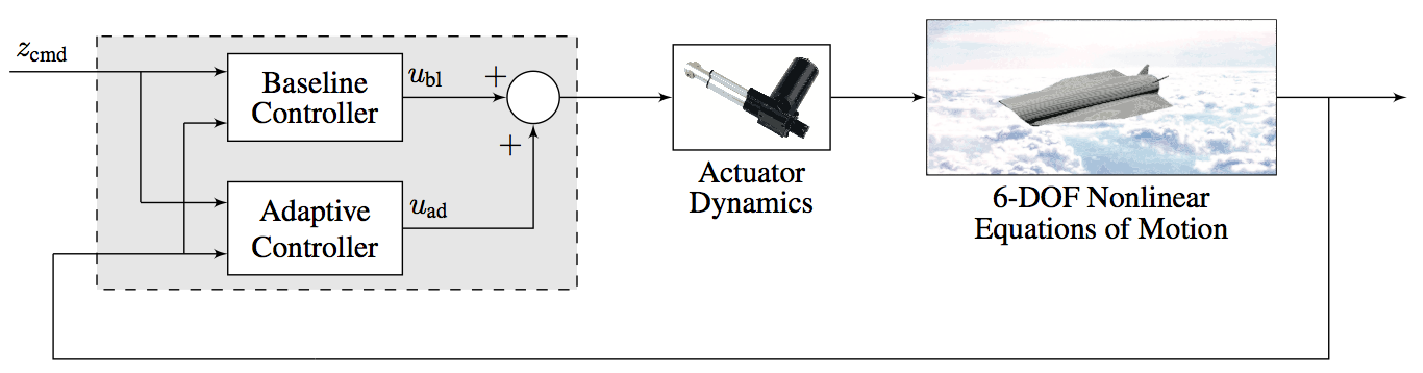
\includegraphics[width=4.5in]{\figurepath/gnc2015_simulation_block.pdf}
      \vspace{-0.1in}
      \caption{Simulation block diagram: evaluation model.\label{fig.block}}
    \end{center}
  \end{figure}

  A $45$ degree roll angle command was given, while commanding zero pitch rate.
  Figure~\ref{fig.nominal} shows the response of the nominal system, with no uncertainty and only the baseline control law: $\Theta=0$.
  Figure~\ref{fig.baselineuncertain} shows the response of the the system with the above uncertainty introduced and only the baseline controller: $\Theta=0$.
  Figure~\ref{fig.adaptive} shows the response of the system with the uncertainties when the adaptive augmentation is used.

  The baseline control law applied to the nominal linear system provides good stability margins and closed-loop performance on the 6-DOF nonlinear evaluation model as shown in Figure~\ref{fig.nominal}.
  The system has a small rise time, minimal overshoot, and a small settling time.
  With the baseline control law only, introduction of the uncertainties causes greater initial overshoot, followed by significant high frequency oscillations, ultimately leading to instability and loss of the aircraft, as shown in Figure~\ref{fig.baselineuncertain}.
  The use of the adaptive component in the control law recovers the baseline control performance, as shown in Figure~\ref{fig.adaptive}.
  When using the adaptive controller, both the control deflections and rates are well within acceptable limits.

  \begin{figure}[H]
    \begin{center}
      \includegraphics[width=6.0in]{\figurepath/gnc2015_nonlin_both_nominal_v2N.eps}
      \vspace{-0.1in}
      \caption{Time response of the nominal system: baseline controller with no uncertainty.\label{fig.nominal}}
    \end{center}
  \end{figure}

  \begin{figure}[H]
    \begin{center}
      \includegraphics[width=6.0in]{\figurepath/gnc2015_nonlin_both_uncertain_v2N.eps}
      \vspace{-0.1in}
      \caption{Time response of baseline control applied to uncertain plant.\label{fig.baselineuncertain}}
    \end{center}
  \end{figure}

  \begin{figure}[H]
    \begin{center}
      \includegraphics[width=6.0in]{\figurepath/gnc2015_nonlin_both_adaptive_v2N.eps}
      \vspace{-0.1in}
      \caption{Time response of baseline controller with adaptive augmentation applied to uncertain plant.\label{fig.adaptive}}
    \end{center}
  \end{figure}

  \section{Conclusion}

  This paper has proposed a new alternative method for synthesizing a CRM based output feedback adaptive controller for a class of uncertain MIMO systems which do not have any unstable transmission zeros.
  The controller is composed of a baseline control gain augmented with an adaptive component to accommodate control effectiveness uncertainty and matched plant uncertainty, and makes use of the closed-loop reference model to improve the transient properties of the overall adaptive system.
  The adaptive controller requires the underlying error dynamics be made SPR through the synthesis of the postcompensator $S_{1}$ and CRM gain $L$, and the SPR relationship is enforced by reducing an underlying bilinear matrix inequality to a feasible linear matrix inequality through appropriate selection of a tuning matrix $X$.
  The procedure does not require the plant first be squared-up.
  It is computationally simple, and it requires only the calculation of some generalized inverses, the solution of the Lyapunov equation, and the solution of a reduced order state feedback problem.
  This procedure is summarized in eight straightforward steps.
  Furthermore, the degrees of freedom in the tuning matrix $X$ capture a large subset of all possible solutions which ensure the SPR property.
  Using these degrees of freedom, $X$ can be tuned to provide the desired stability margins for the baseline system, and a globally stable update law.
  The result is a baseline output feedback controller with good stability margins and adaptive augmentation capable of accommodating matched uncertainties.

  This resulting robust baseline output feedback controller with adaptive augmentation is shown in simulation to provide good tracking performance when applied to a 6-DOF simulation of a hypersonic vehicle with significant uncertainty in control effectiveness, CG shift, and the rolling moment coefficient.
  The simulation results showed that for this uncertainty the robust baseline controller alone was unable to maintain stability, whereas the adaptive controller recovered nominal performance even with the presence of unmodeled actuator dynamics.

  \section*{Appendix A:\ Longitudinal Subsystem Numerical Data}\label{sec.appendix_long}

  The nominal longitudinal plant matrices for a flight condition of Mach 6 at an altitude of 80,000 feet are:
  \begin{equation*}
    A_{p}=
    \left[
    \begin{array}{cccc}
      -0.2398 & 1.0000 \\
      4.5689 & -0.1189
    \end{array}\right]
    \hspace{0.5in}
    B_{p}=
    \left[
    \begin{array}{ccccc}
      -0.0001 \\
      -0.18561
    \end{array}\right]
    \hspace{0.5in}
    C_{p}=
    \left[
    \begin{array}{ccccc}
      0 & 1
    \end{array}\right]
    \hspace{0.5in}
    C_{pz}=
    \left[
    \begin{array}{ccccc}
      0 & 1
    \end{array}\right]
  \end{equation*}

  The following weighting matrices were used to compute $K_{x}$ as in Eq.\ \eqref{eqn.ubl} using the \textsc{Matlab} command \texttt{lqr}
  \begin{align*}
    Q_{\text{lqr}}&=\text{diag}\bigr(
    [\; 0, \; 0.3, \; 170 \; ]\bigr) \\
    R_{\text{lqr}}&=0.0001
  \end{align*}

  \section*{Appendix B:\ Lateral Subsystem Numerical Data}\label{sec.appendix_latr}

  The nominal lateral-directional plant matrices for a flight condition of Mach 6 at an altitude of 80,000 feet are:
  \begin{empheq}[]{alignat*=2}
    A_{p}&=
    \left[
    \begin{array}{cccc}
      -0.0699 & -0.0105 & -1.0000 & 0.0053 \\
      -1331.0 & -2.0308 & -0.0076 & 0 \\
      1.9465 & -0.0016 & -0.0533 & 0 \\
      -0.0002 & 0.8536 & 0 & 0 \\
    \end{array}\right]
    \hspace{0.5in}
    & B_{p}&=
    \left[
    \begin{array}{ccccc}
      0 & 0.0002 \\
      -8.1073 & 10.4560 \\
      0.0320 & -0.2884 \\
      0 & 0 \\
    \end{array}\right] \\
    C_{p}&=
    \left[
    \begin{array}{ccccc}
      0 & 1 & 0 & 0 \\
      0 & 0 & 1 & 0 \\
      0 & 0 & 0 & 1
    \end{array}\right]
    & C_{pz}&=
    \left[
    \begin{array}{ccccc}
      0 & 0 & 0 & 1
    \end{array}\right]
  \end{empheq}

  The following weighting matrices were used to compute $K_{x}$ as in Eq.\ \eqref{eqn.ubl} using the \textsc{Matlab} command \texttt{lqr}
  \begin{align*}
    Q_{\text{lqr}}&=\text{diag}\bigr(
    [\; 0, \; 0.2, \; 40, \; 0, \; 0.2 \; ]\bigr) \\
    R_{\text{lqr}}&=\text{diag}\bigr(
    [\;0.005,\;0.005]\bigr)
  \end{align*}

  \section*{Acknowledgments}

  This research is funded by the Air Force Research Laboratory/Aerospace Systems Directorate grant FA 8650--07--2--3744 for the Michigan/MIT/AFRL Collaborative Center in Control Sciences and the Boeing Strategic University Initiative. Approved for Public Release; Distribution Unlimited. Case Number 88ABW--2014--2551.

  \section*{References}

  \bibliography{\bibsourcepath}
  \bibliographystyle{../sty/aiaa}

\end{document}
